\chapter{Results}\label{ch:results}
% \newthought{Synopsis}\synopsisMethod
The results of the testing of the proof of concept rig are presented in this chapter. The results are presented in a qualitative manner as the rig was not designed to provide quantitative results.
The goal of the testing was to determine if the proof of concept rig was able to simulate the coaptation of the tricuspid valve and the flow of blood through the valve, if the valve leaflets and chordae tendineae could sustain the systolic pressure developed from coaptation, verifying the functionality of the valve for use in the right-heart simulator and later integration of CroiValve DUO.


\section{Proof of Concept Test}
\newthought{Test Procedure}\\
Once leaks were sealed and air bubbles removed, the pulsatile flow loop was started. The pulsatile pump had a set displacement of 50 ml and a frequency of 70 bpm.
This was sequenced every 20 cycles as the system leaks introduced new air bubbles as the testing progressed.
The valve was observed for coaptation and the flow of fluid through the valve was observed.
To measure the cyclic tensile strength of the chordae tendineae, the test was let to run for 10 minutes.



\section{Observations and Qualitative results}
A number of photographs and videos were taken as the testing was conducted.

\begin{figure}[t]
    \begin{fullwidth}
        \centering
        \subfloat[Head-On View]{%
            \href{https://drive.google.com/file/d/1epMX5xH8P03QeNA2DaLtc610iFQK58KK/view?usp=sharing}{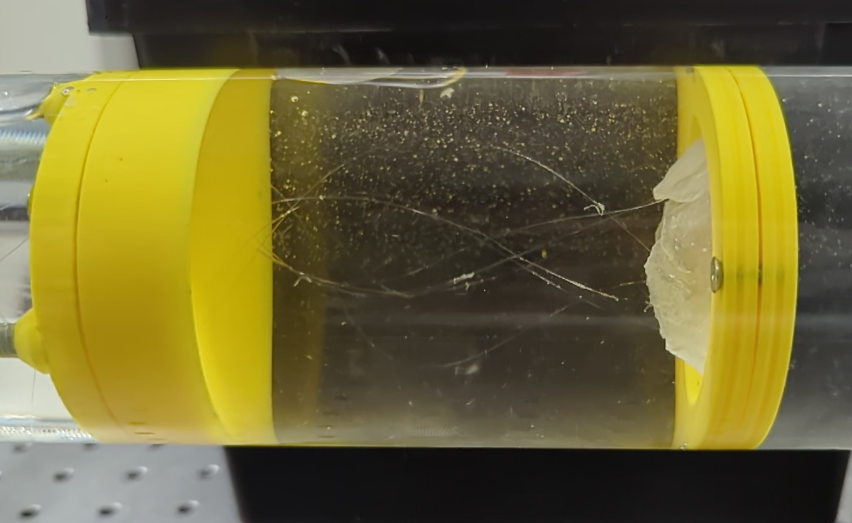
\includegraphics[width=0.45\linewidth]{figures/valverigcloseup}}%
        }\quad
        \subfloat[Oblique View]{%
            \href{https://drive.google.com/file/d/1RXlcIPh9iO5SNXvG8wYL6XBqwaXyd4fS/view?usp=sharing}{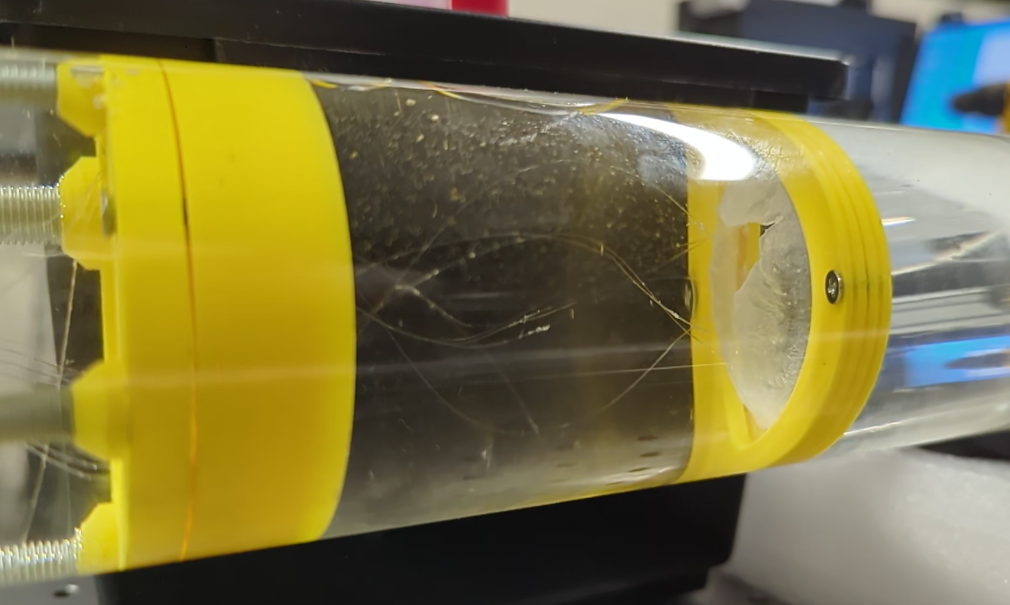
\includegraphics[width=0.45\linewidth]{figures/valverigcloseup2}}
        }
        \caption{Frame from video of valve coapting during testing \textbf{(click to view video)}}
        \label{fig:Videos}
    \end{fullwidth}
\end{figure}